% The Finite Element Method

\section{Introduction}
% <<<

% --- Change: Introduce Poisson's equation first, then give the FDM example for the Poisson equation. Then solve Poisson by FEM.

Among the fundamental PDEs
are the heat equation
    $$\Part{u}{t} = \Delta u + g$$
and the Poisson equation
\begin{equation}\label{poisson_compact}
    -\Delta u = g.
\end{equation}
The latter can be thought of as the steady-state version of the former. The solution of a Poisson problem will be a crucial component
for the solution of the Stokes equations, and since Poisson's equation is likely the simplest non-trivial PDE, it seems ideal to start by discussing
discretization methods for the Poisson equation \eqref{poisson_compact} in particular.


\subsection{Ideas for discretization}
\subsubsection{Discretizing the differential form of the PDE}
It is a theorem of Gauss that in Euclidean space $\mathbb{R}^3$ we have
\begin{equation}\label{gauss_euclidean_divergence}
    \nabla \cdot v = \Part{v_x}{x} + \Part{v_y}{y} + \Part{v_z}{z},
\end{equation}
and we get \eqref{poisson_compact} in the form
\begin{equation}\label{poisson_differential_intro}
    -\left(\frac{\partial^2 u}{\partial x^2}
           +\frac{\partial^2 u}{\partial y^2}
           +\frac{\partial^2 u}{\partial z^2}\right) = g.
\end{equation}
Thinking about \eqref{poisson_differential_intro} leads to the finite difference method, historically the first and
still very important in applications.
This form immediately indicates an effective method
of discretization, by forming secant approximations of the derivatives over a regular grid. The approximate solution is then
represented as a function of this grid.
However, it may be hard to give a real interpretation of what the solution samples at grid points say about the solution everywhere.
They could be a coefficients of, for example, hat basis functions.
Yet a finite difference discretization of \eqref{continuity_equation_differential} may not take this into account at all. One might feel that
limits have been taken too soon.

% Consider a single conservation law as described in section \ref{conservation_laws}. This law
% was given in two forms, ``integral'' \eqref{continuity_equation}:
% \begin{equation*}
%     \frac{d}{dt} \int_{\Omega_0} \phi\,dx = \int_{\Omega_0} s\,dx + \int_{\pomn} \phi j \cdot \left(-\hat{n}\right)\,dx,
% \end{equation*}
% and ``differential'' \eqref{continuity_equation_differential}:
% \begin{equation*}
%     \Part{\phi}{t} = s - \nabla\cdot (\phi j).
% \end{equation*}

\subsubsection{Discretizing the integral form of the PDE}
In physics, Poisson's equation is an equilibrium conservation law, and therefore has an integral form.
This form will give clearer routes to discretizations which
have geometric meaning.
% Thinking instead about \eqref{poisson_integral_intro} will lead to Galerkin methods, which include finite volumes, finite elements, and spectral methods.
For example, the general integral conservation law \eqref{continuity_equation},
\begin{align*}
    \frac{d}{dt} \int_{\Omega_0} \phi\,dx = \int_{\Omega_0} s\,dx + \int_{\pomn} \phi j \cdot \left(-\hat{n}\right)\,dx,
\end{align*}
is a geometric statement about fluxes
of quantity $\phi$ by $j$, quantified over arbitrary control volumes $\Omega_0$.
We have an infinite number of control volumes, and therefore an infinite number of equations which must hold, and an infinite-dimensional
space of solutions to choose from. A key idea, then, is to choose a finite number of equations and a finite-dimensional subspace of possible solutions.
A supposed solution will be represented by the coefficients of some choice of basis functions for the subspace. Each equation will be checked exactly against this supposed solution.

\vskip 0.2in
(figure)
\vskip 0.2in

Finite element methods, and more generally Galerkin methods, live comfortably in the language of weak solutions, integral forms of partial differential equations,
and the calculus of variations.
To continue with this idea, we must write the Poisson equation \eqref{poisson_compact} in integral form.

\subsection{Deriving the Poisson equation through diffusion processes}
% <<<
A diffusion process ``levels out'' some quantity, such as temperature or some chemical concentration. We can intuitively think of a diffusion as a
progressive ``blurring''
such as in a camera defocus, and in fact many common image processing techniques use diffusion PDEs from physics \cite{tum}. We will stick with
the notion of temperature $h$ as the diffused quantity.
\textit{Fick's law of diffusion} is a constitutive relation giving the bulk flux of temperature $h$ as proportional to the negative gradient:
    $$hj = -\mu\nabla h,$$
where $\mu$ is called the diffusion coefficient.
This is one way of saying that the temperature tends to level out.
If we form a continuity equation \eqref{continuity_equation} for temperature, with source $s$, we get
\begin{equation}\label{heat_equation_integral}
    \frac{d}{dt} \int_{\Omega_0} h\,dx = \int_{\Omega_0} s\,dx + \int_{\pomn} \mu \nabla h \cdot \hat{n}\,dx,
\end{equation}
which by application of Stokes' theorem becomes
\begin{equation}\label{heat_equation_differential}
    \frac{dh}{dt} = s + \nabla \cdot \left(\mu \nabla h\right).
\end{equation}
If we further assume that the diffusion coefficient $\mu$ is constant, we get
\begin{equation}\label{heat_equation_differential_constant}
    \frac{dh}{dt} = s + \mu\nabla \cdot \nabla h = s + \mu\Delta h,
\end{equation}
which is the standard heat equation.
The steady-state heat equation is then
\begin{equation}\label{poisson_equation}
    -\Delta h = f,
\end{equation}
where we let $f = s/\mu$ in the above. Equation \eqref{poisson_equation} is called the Poisson equation,
which models steady-state diffusion processes and can be used to calculate gravitational or electrostatic potential fields.
In integral form, ``undoing'' the application of Stokes' theorem above, the Poisson equation is
\begin{equation}\label{poisson_equation_integral}
    \int_{\pomn} -\nabla h\cdot \hat{n}\,dx = \int_{\omn} f\,dx.
\end{equation}
Form \eqref{poisson_equation_integral} clearly shows that we are calculating a steady state,
as we are solving for $h$ such that the amount of heat that leaves $\Omega_0$ is the amount created by the source function.
This form will be the most convenient for our numerical methods.
% >>>

\subsection{Discretizing the Poisson equation}\label{discretizing_poisson}
% <<<
Equation \eqref{poisson_equation_integral} is quantified over arbitrary control volumes $\Omega_0$.
A simple idea is to break the domain $\Omega$ up into small cells $\Omega_1,\cdots,\Omega_n$, and check that the flux integral holds over each of these.
We will then have $n$ equations on $h$. As this system will be underdetermined ($h$ has infinite degrees of freedom), we must
restrict $h$ to what we will call a ``test space'',
    $$\Phi = \text{span}\left\{\phi_1,\cdots,\phi_n\right\}.$$
The basis functions $\phi_i$ should generate a ``good'' space of approximations,
such that our linear system is non-singular.
We then have a discrete system of equations
\begin{align*}
    \int_{\pom_j} -\nabla \left(\sum_{i=1}^n h_i\phi_i\right)\cdot \hat{n}\,dx = \int_{\om_j} f\,dx,\quad j=1,\cdots,n.
\end{align*}
By linearity, to emphasize the separate integrals that need to be computed, the above equation can be written as
\begin{equation}\label{poisson_equation_integral_discretized}
    \sum_{i=1}^n h_i\int_{\pom_j} -\nabla \phi_i \cdot \hat{n}\,dx = \int_{\om_j} f\,dx,\quad j=1,\cdots,n.
\end{equation}
We see here that there must be some restrictions on the $\phi_i$.
Formally, our basis functions must be in the Sobolev space $H^1(\Omega)$. This simply means that they must have a gradient defined ``almost everywhere''.
It does not matter if the gradient is not defined at isolated lower-dimensional subsets, as these make no contribution to
the integral. Since the source $f$, our domain partition $\Omega_j$, and the basis functions $\phi_i$ are known, we can pre-compute
the majority of \eqref{poisson_equation_integral_discretized} to give a matrix system

\newcommand{\integralentry}[2]{\int_{\pom_{#1}}-\nabla\phi_{#2}\cdot\hat{n}\,dx}
\begin{equation}\label{poisson_matrix_equation}
    A\hat{h} = \begin{bmatrix}
            \integralentry{1}{1} & \cdots & \integralentry{1}{n} \\
            \vdots & & \vdots \\
            \integralentry{n}{1} & \cdots & \integralentry{n}{n}
            \end{bmatrix}
    \begin{bmatrix} h_1 \\ h_2 \\ \vdots \\ h_{n-1} \\ h_n \end{bmatrix}
    =
    \begin{bmatrix} \int_{\om_1}f\,dx \\ \int_{\om_2}f\,dx \\ \vdots \\ \int_{\om_{n-1}}f\,dx \\ \int_{\om_n}f\,dx \end{bmatrix}
    = \hat{f}.
\end{equation}
If our domain partition $\Omega_1,\cdots,\Omega_n$ and test space $\Phi = \text{span}\left\{\phi_1,\cdots,\phi_n\right\}$
are chosen well, this linear system will be non-singular and hopefully well-conditioned.
In all cases we have a conservative system of balanced fluxes, but it is another question whether our approximation
$\Phi\hat{h}$ is good.

\subsubsection{Choosing a domain partition and test space}
Possibly the simplest scheme is to triangulate $\Omega$ as
    $\Omega = \biguplus T_i$
such that we have $n$ nodal points.
Each nodal point $p_i$ will be associated with a piecewise ``hat'' basis function $\phi_i$ which is $1$ at $p_i$ and
$0$ at its neighbours.

\vskip 0.2in
(draw this)
\vskip 0.2in

As we typically have more triangles than vertices, we cannot use the $T_i$ as our domain partition. However, we may
associate to each $p_i$ a domain $\Omega_i$ called the \textit{Voronoi cell}.

\vskip 0.2in
(draw this)
\vskip 0.2in

This scheme has found some success, especially in the domain of geometry processing \cite{polygon_mesh_processing}.
By Stokes' theorem, the matrix $A$ in \eqref{poisson_matrix_equation} can be thought of as a negative discrete Laplacian.
If we compute these integrals, we will find a very simple closed form for the entries of $A$.

In geometry processing this matrix is called the ``cotangent Laplacian'' \cite{polygon_mesh_processing}, and it is typically
applied to surface meshes in $\mathbb{R}^3$, which can be thought of as triangulations of a smooth surface.

\subsubsection{Results and visualisation}
\vskip 0.2in
(results and visualisation)
\vskip 0.2in
We have worked through an instance of a \textit{finite volume method} \cite{pde_larsson}.
Finite volume methods are characterised by an exact domain partition and computation of flux integrals.
Finite volume methods are typically \textit{conservative}, due to the ``flux network'' nature of the discretisation.
% >>>
\subsection{The notion of a trial function}\label{trial_function}
% <<<
The matrix equation \eqref{poisson_matrix_equation} consists of linear equations
\begin{align*}
    \int_{\pom_1} -\nabla \left(\sum_{i=1}^n h_i\phi_i\right) \cdot \hat{n}\,dx
    =
    \int_{\om_1}f\,dx,
\end{align*}
and so on. We cannot compute flux integrals
over all arbitrary control volumes, but we can take a number of ``trial'' flux integrals over the finite number of cells $\Omega_i$.
We can take linear combinations of these equations to get more equations which must hold on a solution.
For example,
\begin{equation}\label{example_trial_sum}
    \int_{\pom_1} -\nabla \left(\sum_{i=1}^n h_i\phi_i\right) \cdot \hat{n}\,dx
    +
    \int_{\pom_2} -\nabla \left(\sum_{i=1}^n h_i\phi_i\right) \cdot \hat{n}\,dx
    =
    \int_{\om_1}f\,dx
    +
    \int_{\om_2}f\,dx
\end{equation}
must hold. At first sight, \eqref{example_trial_sum} cannot directly be interpreted as a statement about a ``flux integral'', but rather about a sum
of flux integrals. However, a key idea is to regard \eqref{example_trial_sum} as a flux integral over a \textit{formal sum} of domains,
    $$\Omega_1 + \Omega_2.$$
We now have the equation
\begin{equation}
    \int_{\pom_1 + \pom_2} -\nabla \left(\sum_{i=1}^n h_i\phi_i\right) \cdot \hat{n}\,dx
    =
    \int_{\om_1 + \om_2}f\,dx.
\end{equation}
Formally $\Omega_1 + \Omega_2$ is called a \textit{chain}. For example, we may visualise $\Omega_1 + 2\Omega_2 + 0.5\Omega_4$ as:

\vskip 0.2in
(draw this)
\vskip 0.2in

We define the boundary operator $\partial$ to be linear in formal sums e.g.,
    $$\partial(\Omega_1 + \Omega_2) = \pom_1 + \pom_2.$$
If $\om_1$ and $\om_2$ share a boundary, we would like $\om_1 + \om_2$ to represent their union, such that a flux
integral over $\partial(\Omega_1 + \Omega_2)$ evaluates to zero on the shared boundary. This can be done by thinking of
the boundary as \textit{oriented}, as in, consisting of oriented ``surface elements'' over which flux integrals can be taken.
For example, the $\hat{n}$ in a flux integral denotes the outward-pointing normal, which represents an ``outward-flux-measuring surface element''.
The opposite $-\hat{n}$ then represents the ``inward-flux-measuring surface element'', which is outward from the perspective of an adjacent cell.

\vskip 0.2in
(draw this)
\vskip 0.2in

We may now define
    $$\Psi = \text{span}\left\{\Omega_1,\cdots,\Omega_n\right\}$$
to be the \textit{trial space}, where the span is taken with respect to formal sums. As with a typical linear space,
we may choose from many possible bases. For example,
    $$\Psi = \text{span}\left\{\Omega_1, \Omega_2, \Omega_3\right\} =
    \text{span}\left\{\Omega_1 + \Omega_2, 2\Omega_2, \Omega_3\right\}.$$
A key idea, leading to Galerkin methods, is to allow freedom in the choice of our trial space $\Psi$.
Notably, we do not need $\Psi$ to be a space of formal sums of domains.
The Poisson equation is discretised over flux integrals around cell boundaries in the linear system \eqref{poisson_equation_integral_discretized},
which we repeat here:
\begin{align*}
    \sum_{i=1}^n h_i\int_{\pom_j} -\nabla \phi_i \cdot \hat{n}\,dx = \int_{\om_j} f\,dx,\quad j=1,\cdots,n.
\end{align*}
Applying Stokes' theorem, we get
\begin{align*}
    \sum_{i=1}^n h_i\int_{\om_j} -\Delta \phi_i \,dx = \int_{\om_j} f\,dx,\quad j=1,\cdots,n.
\end{align*}
We can think of these integrals as over the \textit{entire domain} $\Omega$, giving the form
\begin{align*}
    \sum_{i=1}^n h_i\int_{\om} -\Delta \phi_i\cdot \chi(\om_j)\,dx = \int_{\om} f\cdot\chi(\om_j)\,dx,\quad j=1,\cdots,n.
\end{align*}
where $\chi(\om_j)$ is the indicator function of $\om_j$,
\begin{align*}
    \chi(\om_j)(x) \coloneqq \left\{\begin{array}{lr}
        0 &\text{if $x \in \om_j$}\\
        1 &\text{if $x \notin \om_j$.}\\
        \end{array}\right.
\end{align*}
Note that we can now think of our trial space $\Psi$ as a span of functions, instead of a span of domains:
    $$\Psi = \text{span}\left\{\chi(\Omega_1),\cdots,\chi(\Omega_n)\right\}.$$
Now we can instead let
    $$\Psi = \text{span}\left\{\psi_1,\cdots,\psi_n\right\}$$
where the $\psi_j$
need not be the indicator functions of a domain partition. We now have the system of equations
\begin{align*}
    \sum_{i=1}^n h_i\int_{\om} -\Delta \phi_i \psi_j\,dx = \int_{\om} f\psi_j\,dx,\quad j=1,\cdots,n.
\end{align*}
By integration by parts we have
\begin{equation}\label{poisson_galerkin}
    \sum_{i=1}^n h_i\int_{\om} -\nabla \phi_i \cdot \nabla \psi_j\,dx = \int_{\om} f\psi_j\,dx,\quad j=1,\cdots,n,
\end{equation}
and we see that we still only require the $\phi_i$ to be in $H^1(\Omega)$.
We can see that equation \eqref{poisson_galerkin} is very similar to the exact fluxes in \eqref{poisson_equation_integral_discretized}.
There is a real geometric sense in which \eqref{poisson_galerkin} is a ``blurred convolution'' of flux integrals.

\subsubsection{Integrating over trial functions versus integrating over domains}
The reasoning here is in the spirit of Green's functions.
While this is more readily formalised with the notion of a distribution, or generalised function, we will work with the Dirac delta function,
defined by
\begin{align*}
    \int_{\omn} \delta_y\,dx = 
    \left\{\begin{array}{lr}
        1 &\text{if $y \in \omn$}\\
        0 &\text{otherwise}.\\
        \end{array}\right.
\end{align*}
For example, possibly under some regularity assumptions, we may represent a trial function $\psi_j$ on $\Omega$ as
    $$f = \int_\Omega \delta_x f(x)\,dx,$$
which we may call ``Riemann-integral-like''.
We may instead represent $\psi_j$ in a ``Lebesgue-integral-like'' way by defining
    $$L_y(\psi_j) \coloneqq \left\{z \in \Omega \mid \psi_j(z) = y\right\}$$
to be a level set of $\psi_j$, the points of $\Omega$ for which $\psi_j = y$. We can then express $\psi_j$ as
    $$\psi_j = \int_{-\infty}^\infty \left[\int_{L_y(\psi_j)} y\delta_x \,dx\right]\,dy.$$
This gives $\psi_j$ as the totality of its level sets.
For example, if we let $\Psi$ be spanned by the hat functions on some triangulation, each hat function $\psi_j$
can be thought of as a totality of level sets culminating in the point-set of $\psi_j(p_j) = 1$.

\vskip 0.2in
(draw this)
\vskip 0.2in

The discretised Poisson equation \eqref{poisson_galerkin} involves an integral over $\nabla \phi_i \cdot \nabla \psi_j$,
and we can compute this as
\begin{equation}\label{flux_convolution}
\begin{split}
    \int_{\om} \nabla \phi_i \cdot \nabla \psi_j\,dx
        &= \int_{-\infty}^\infty \int_{\om} \nabla\phi_i \cdot \nabla\left[\int_{L_y(\psi_j)} y\delta_z \,dz\right]\,dx\,dy\\
        &= \int_{-\infty}^\infty y \int_{L_y(\psi_j)} \nabla\phi_i \cdot \hat{n}\,dx\,dy.
\end{split}
\end{equation}
We have this final equality by noting that the gradient of $\psi_j$ at $x$, where $\psi_j(x) = y$, is orthogonal to the level set $L_y{(\psi_j)}$,
and has length $y$:

\vskip 0.2in
(draw this)
\vskip 0.2in

We can think of the ``flux trial'' \eqref{poisson_galerkin} as involving ``blurred fluxes'' as in \eqref{flux_convolution}.
For example, if we let $\Phi = \Psi$ be the set of hat functions on some triangulation
of $\Omega$, then form and solve the matrix system, we get a generally non-conservative system of fluxes. We have lost conservativeness
by the ``blurring'' of the flux integrals, but we may have gained advantages in terms of stability and convergence: in this case,
the linear system will be symmetric-positive-definite, and stably solvable by, for example, conjugate gradients.

\subsection{Implementing FEM for Poisson's equation}

We have so far worked up to an instance of a \textit{finite element method}.
Finite element methods are characterised by a test space $\Phi$ and trial space
$\Psi$ with basis functions of \textit{compact support}, where $\Phi$ and $\Psi$ typically consist of continuous functions in
some Sobolev space, constructed over a domain tessellation. We will formally define a ``finite element method'', following Ciarlet \cite{ciarlet},
after one more example, the steady Stokes equations.

\begin{center}
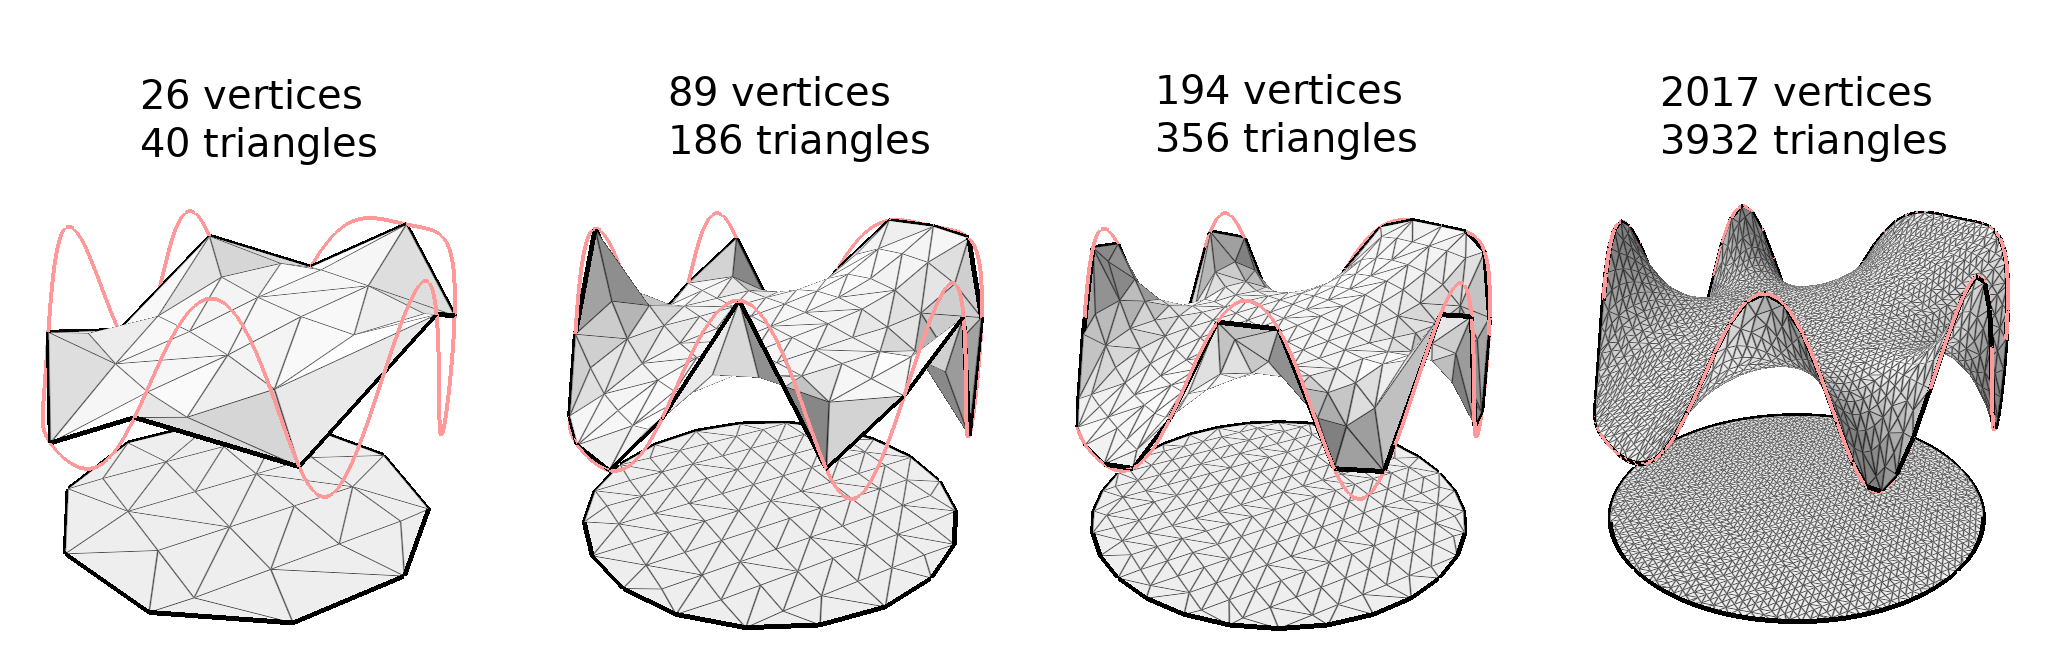
\includegraphics[width=\linewidth]{figures/laplace/laplace.png}
\end{center}


% \subsubsection{Duality and differential geometry}
% Again, the trial space $\Psi$ needs not be formed by indicator functions of domains.
% To see this more clearly, we can emphasize the duality between chains and the functions integrated over them by using inner product notation, or ``duality pairing'':
% \begin{equation}
%     \inner{-\nabla \left(\sum_{i=1}^n h_i\phi_i\right), \partial\left(\sum_{i=1}^n \omega_i \Omega_i\right)^\perp}
%     =
%     \inner{f, \sum_{i=1}^n \omega_i \Omega_i}.
% \end{equation}
% The duality pairing is an integral over the whole domain, where pieces of chains (such as the ``surface elements'' in a flux integral) are
% paired with pieces of function data of the same dimension (such as the heat gradient, or the source function).
% We can write our original (weak) Poisson problem \eqref{poisson_equation_integral} in this notation as
% \begin{align*}
%     \inner{-\nabla h, \pomn^\perp}
%     =
%     \inner{f, \omn}.
% \end{align*}
% for arbitrary control volumes $\Omega_0$. The $\perp$ symbol denotes an orthogonal complement, as
% we would like to pair gradient vectors with \textit{normals} to the boundary rather than the boundary elements themselves,
% as we are calculating total fluxes. More formally, in differential
% geometry, this should be denoted by the ``Hodge star'' operator $\star$, which we will use from now on, as
% it will be convenient to think of the orthogonal complement as an operator acting by multiplication:
% \begin{equation}\label{poisson_duality}
%     \inner{-\nabla h, \star\pomn}
%     =
%     \inner{f, \omn}.
% \end{equation}
% By Stokes' theorem we have the form
% \begin{align*}
%     \inner{-\nabla \cdot \nabla h, \omn}
%     =
%     \inner{f, \omn}.
% \end{align*}
% The duality pairing is in fact an inner product, so we see that operator
% $\star\partial$ is \textit{adjoint} to $\nabla\cdot$.
% This is exactly what Stokes' theorem was created to say, albeit expressed in a more abstract language.
% We may ask why we must restrict the chain to be an indicator function. Why not ``integrate against'' some other function,
% \begin{align*}
%     \inner{-\nabla \cdot \nabla h, \psi}
%     =
%     \inner{f, \psi}?
% \end{align*}
% Yet does the form
% \begin{align*}
%     \inner{-\nabla h, \star\partial \psi}
%     =
%     \inner{f, \psi}
% \end{align*}
% make sense?
% >>>
% >>>

\section{Solving the Stokes equations}
% <<<
% Introduction 
% <<<
The Stokes equations \eqref{unsteady_stokes}, which are solved for a stable incompressible Navier-Stokes flow,
assume the Reynolds number is $Re \ll 1$ and thus convective processes are neglible in comparison to viscous processes.
We will begin with the steady-state form \eqref{steady_stokes}.
Due to this simplification, the Steady stokes equations \eqref{steady_stokes}, repeated here:
\begin{align*}
    \mu\Delta u + \rho g - \nabla p = 0,\quad \nabla\cdot u = 0,
\end{align*}
form a constrained linear equation. As we saw in section \ref{pressure_derivation}, the pressure term $p$ is a Lagrange multiplier introduced
with the constraint $\nabla\cdot u = 0$. We will begin by discretizing the \textit{unconstrained} steady Stokes equations,
which are a vector Poisson equation:
\begin{equation}\label{steady_stokes_unconstrained}
    -\mu\Delta u = \rho g.
\end{equation}
% >>>
\subsection{Discretizing the vector Poisson equation}\label{discretizing_vector_poisson}
% <<<
In principle we should keep the Stokes equation
in integral form (using the conservative-form Cauchy momentum equation \eqref{cauchy_continuity_eulerian}), and continue as we did
in section \ref{trial_function}. However,
we will take a formal step to skip the reasoning of section \ref{trial_function}, typical of finite element method derivations.
As we start with the \textit{differential} equation \eqref{steady_stokes_unconstrained}, we can introduce a trial space $\Psi$ and then ``weaken''
the equation by integrating against $v \in \Psi$, and removing the Laplacian by integration by parts:
\begin{equation}\label{steady_stokes_unconstrained_weak}
    \int_\Omega -\mu\Delta u\cdot v\,dx = \int_\Omega \rho g\cdot v\,dx
    \quad\equiv\quad
    \int_\Omega -\mu\nabla u : \nabla v\,dx = \int_\Omega \rho g\cdot v\,dx.
\end{equation}

Noting that the left-hand-side of \eqref{steady_stokes_unconstrained_weak} is a bilinear form in $u$ and $v$, and the right-hand-side
is a linear functional in $\psi$, it is standard practice (ref) to write this kind of equation as
\begin{equation}
    a(u, v) = f(v).
\end{equation}
Our subsequent derivations are much the same as in \ref{discretizing_poisson}, simplified by our new notation.
We can now approximate $u$ in the test space $\Phi$ as $\hat{u} = \sum_{i=1}^nu_i\phi_i$. By linearity we only need to compute
trials over the basis trial functions $\psi_j$.
We then have the linear system of equations
\begin{equation}\label{elliptic_bilinear_form}
    \sum_{i=1}^n u_i a\left(\phi_i, \psi_j\right) = f(\psi_j),\quad j=1,\cdots,n,
\end{equation}
which can be written in matrix form as
\begin{equation}\label{elliptic_bilinear_form_matrix}
    A\hat{u} = \begin{bmatrix}
            a(\phi_1, \psi_1) & \cdots & a(\phi_1, \psi_n) \\
            \vdots & & \vdots \\
            a(\phi_n, \psi_1) & \cdots & a(\phi_n, \psi_n)
            \end{bmatrix}
    \begin{bmatrix} u_1 \\ u_2 \\ \vdots \\ u_{n-1} \\ u_n \end{bmatrix}
    =
    \begin{bmatrix} f(\psi_1) \\ f(\psi_2) \\ \vdots \\ f(\psi_{n-1}) \\ f(\psi_{n}) \end{bmatrix}
    = \hat{f}.
\end{equation}
% The matrix $A$ is symmetric positive-definite, and we can therefore think of a solution to \eqref{elliptic_bilinear_form_matrix}
% as as a minimizer of the scalar quadratic form
% \begin{equation}\label{elliptic_quadratic_form}
%     \hat{E}(\hat{u}) \coloneqq \frac{1}{2} \inner{\hat{u}, A\hat{u}} - \inner{\hat{u}, \hat{f}}.
% \end{equation}
% This is simply a discrete realisation of the fact that we can, as described in section \ref{pressure_derivation}, think
% of a solution to the vector Poisson equation as a minimizer of the Dirichlet energy \eqref{steady_stokes_dirichlet_energy},
% \begin{align*}
%     E(u) \coloneqq \int_{\Omega} \frac{\mu}{2} \inner{\nabla u, \nabla u} - \rho g\cdot u \,dx.
% \end{align*}
We can solve \eqref{elliptic_bilinear_form_matrix} to get a velocity field $\sum_{i=1}^n u_i\phi_i$, although in general this will not satisfy $\nabla\cdot u = 0$.
As some preliminary analysis, if $\Phi = \Psi$ and have the same basis functions, we have a symmetric-positive-definite system. This form of linear system is known to be stably solvable,
for example by the conjugate gradient method.
% >>>
\subsection{Discretizing the steady Stokes equations}\label{discretizing_steady_stokes}
% <<<
As described in section \ref{pressure_derivation}, the pressure $p$ is a Lagrange multiplier that appears
when solving the optimization problem \eqref{stokes_flow_optimization}:
\begin{equation*}
\begin{aligned}
& \underset{u}{\text{minimize}}
& & E(u) =  \frac{\mu}{2} \inner{\nabla u, \nabla u} - \inner{u, \rho g}\\
& \text{subject to}
& & \nabla\cdot u = 0.
\end{aligned}
\end{equation*}

\newcommand{\trialconstraint}{{\Psi_{\text{constraint}}}}
\newcommand{\testpressure}{{\Phi_{\text{pressure}}}}
As a first idea, we can introduce $p$ as a variable to solve for. Solving for the pressure (the ``dual variable'') simultaneously with the velocity
(the ``primal variable'')
is called a primal-dual method for the optimization \eqref{stokes_flow_optimization}, and the resulting finite element method is called \textit{mixed}.
Pressure then needs to be discretized, so we introduce another test space $\testpressure$.
To get a weak form of the steady Stokes equations \eqref{steady_stokes}, which are two equations including the constraint $\nabla\cdot u = 0$, we introduce
another trial space $\trialconstraint$, whose functions will be integrated against $\nabla\cdot u$. The weak form is then
\begin{equation*}
\begin{split}
    &\int_\om \left(\mu\Delta u + \rho g - \nabla p\right)\cdot v\,dx = 0,\\
    &\int_\om \left(\nabla\cdot u\right) q\,dx = 0, \quad\text{where $v \in \Psi, q \in \trialconstraint$},
\end{split}
\end{equation*}
which by integration by parts can be written as
\begin{equation}\label{steady_stokes_weak}
\begin{split}
    &\int_\om -\mu\nabla u : \nabla v - \left(\nabla\cdot v\right)p\,dx = \int_\om \rho g\cdot v\,dx,\\
    &\int_\om \left(\nabla\cdot u\right) q\,dx = 0, \quad\text{where $v \in \Psi, q \in \trialconstraint$}.
\end{split}
\end{equation}
As in section \ref{discretizing_vector_poisson}, we introduce notation for the bilinear and linear forms in \eqref{steady_stokes_weak}:
\begin{equation}
\begin{split}
    a(u, v) &\coloneqq \int_\om-\mu\nabla u : \nabla v\,dx,\quad\text{for $u \in \Phi, v \in \Psi$},\\
    \hat{b}(p, v) &\coloneqq \int_\om-\left(\nabla\cdot v\right)p\,dx,\quad\text{for $p \in \testpressure, v \in \Psi$},\\
    b(u, q) &\coloneqq \int_\om-\left(\nabla\cdot u\right)q\,dx,\quad\text{for $u \in \Phi, q \in \trialconstraint$},\\
    f(v) &\coloneqq \int_\om \rho g\cdot v\,dx\quad\text{for $v \in \Psi$}.
\end{split}
\end{equation}
Although they have the same form, $b$ and $\hat{b}$ are distinguished as they take inputs in different function spaces.
We now have a simplified notation for the weak form \eqref{steady_stokes_weak},
\begin{equation}\label{steady_stokes_weak_notation}
\begin{split}
    &a(u, v) + \hat{b}(p, v) = f(v),\\
    &b(u, q) = 0, \quad\text{where $v \in \Psi, q \in \trialconstraint$}.
\end{split}
\end{equation}
% Solving for $u^*$ in the equation $a(u^*, v) = f(v)$ is the standard vector Poisson equation, resulting in a symmetric-positive-definite
% system when the test and trials spaces are discretized. We can imagine letting $p = 0$ and solving for $u^*$.
% The first condition of \eqref{steady_stokes_weak_notation} will hold, but the second condition (does $b(u^*, q) = 0$?) generally will not.
Working with discrete function spaces, we get a $2n\times 2n$ linear system in the unknowns $u_1,\cdots,u_n$ and $p_1,\cdots,p_n$,
\begin{equation}
\begin{split}
    &\sum_{i=1}^n u_i a\left(\phi_i, \psi_j\right) + \sum_{i=1}^np_i\hat{b}\left(\phi^C_i, \psi_j\right) = f(\psi_j),\\
    &\sum_{i=1}^nu_ib\left(\phi_i, \psi^C_j\right) = 0,\quad j=1,\cdots.n.
\end{split}
\end{equation}
To emphasize the linear system structure of \eqref{steady_stokes_weak_notation}, the block matrix form is:
\begin{equation}\label{steady_stokes_matrix}
\def\arraystretch{1.5}
\begin{split}
    M\hat{x}
    &= \begin{bmatrix}
            A & \hat{B} \\
            B & 0
    \end{bmatrix}\hat{x} \\
    &= \left[\begin{array}{@{}ccc|ccc@{}}
            a(\phi_1, \psi_1) & \cdots & a(\phi_1, \psi_n)     & \hat{b}(\phi^C_1, \psi_1) & \cdots & \hat{b}(\phi^C_1, \psi_n) \\
            \vdots & & \vdots                                  & \vdots & & \vdots \\
            a(\phi_n, \psi_1) & \cdots & a(\phi_n, \psi_n)     & \hat{b}(\phi^Cn, \psi_1) & \cdots & \hat{b}(\phi^C_n, \psi_n) \\
            \hline
            b(\phi_1, \psi^C_1) & \cdots & b(\phi_1, \psi^C_n) & 0 &\cdots& 0      \\
            \vdots & & \vdots \\                               & \vdots & & \vdots \\
            b(\phi_n, \psi^C_1) & \cdots & b(\phi_n, \psi^C_n) & 0 &\cdots& 0       
    \end{array}\right]
    \left[\begin{array}{c} u_1 \\ \vdots \\ u_n \\ \hline p_1 \\ \vdots \\ p_n \end{array}\right]
    =
    \left[\begin{array}{c} f(\psi_1) \\ \vdots \\ f(\psi_{n}) \\ \hline 0 \\ \vdots \\ 0 \end{array}\right]
    = \hat{b}.
\end{split}
\end{equation}
\subsubsection{Is this method reasonable?}
For the vector Poisson equation, letting $\Phi = \Psi$, we ended up with a symmetric-positive-definite system \eqref{elliptic_bilinear_form_matrix}, which is known to be stably solvable.
We can ask how reasonable it is to solve \eqref{steady_stokes_matrix}, and what trial and test spaces we should use.
In fact, in the problem \eqref{steady_stokes_weak_notation}, and more generally in a ``saddle point problem'', arising
in Lagrange-multiplier methods for constrained PDEs, we should not choose just any test and trial spaces.
The Ladyzhenskaya--Babu\v{s}ka--Brezzi condition, discussed later, enforces restrictions on choices that result in a stable method.
We will until then continue with computations.

\subsubsection{Results and visualisation}
\vskip 0.2in
(results and visualisation)
\vskip 0.2in
% >>>
\subsection{Discretizing the unsteady Stokes equations}\label{discretizing_unsteady_stokes}
% <<<
\newcommand{\uprev}{{u_{\text{prev}}}}
The steady Stokes above are the stable state of the time-dependent Stokes flow,
after the transient flow behaviour settles down. The unsteady Stokes equations \eqref{unsteady_stokes} are
\begin{equation*}
    \rho\Part{u}{t} = \mu\Delta u + \rho g - \nabla p, \quad \nabla\cdot u = 0.
\end{equation*}
These form an initial-boundary-value problem, and this will be our first attempt at discretizing a PDE in time.
We could think of solving with the test and trial spaces over the domain $\Omega \times [0, T)$, but this is typically not done due to the memory costs,
and different qualitative meaning of the time variable \cite{ham_fem}. Instead, we will use an implicit-Euler finite difference in time: 
\begin{equation}\label{unsteady_stokes_implicit_euler}
    \frac{\rho}{\Delta t} \left(u^{(n)} - u^{(n-1)}\right) = \mu\Delta u^{(n)} + \rho g - \nabla p^{(n)}, \quad \nabla\cdot u^{(n)} = 0,
\end{equation}
where $\Delta t$ is a fixed time step, and $u^{(n)}$ and $p^{(n)}$ is the solution at time $t_n = n\Delta t$. We can weaken each step
\eqref{unsteady_stokes_implicit_euler}
by integrating against trial functions $v \in \Psi$ and $q \in \trialconstraint$, performing integration by parts as in section \ref{discretizing_steady_stokes},
and rearranging the knowns and unknowns. We can also let $u$ be $u^{(n)}$, $p$ be $p^{(n)}$, and $\uprev$ be $u^{(n-1)}$ in the above to simplify
subsequent notation. The weak form of \eqref{unsteady_stokes_implicit_euler} is then:
% \begin{equation}\label{unsteady_stokes_implicit_euler_weak}
% \begin{split}
%     \frac{\rho}{\Delta t} \int_\om \left(u^{(n)} - u^{(n-1)}\right)\cdot v\,dx
%         &= \int_\om \mu\nabla u^{(n)}:\nabla v + \rho g\cdot v + \left(\nabla\cdot v\right) p^{(n)}\,dx,\\
%     \quad \int_\om \left(\nabla\cdot u^{(n)}\right) q\,dx &= 0.
% \end{split}
% \end{equation}
\begin{equation}\label{unsteady_stokes_implicit_euler_weak}
\begin{split}
    \int_\om \frac{\rho}{\Delta t} u\cdot v - \mu\nabla u:\nabla v - \left(\nabla\cdot v\right)p\,dx
        &= \int_\om \frac{\rho}{\Delta t}\uprev\cdot v + \rho g \cdot v\,dx,\\
    \quad \int_\om \left(\nabla\cdot u\right) q\,dx &= 0,
\end{split}
\end{equation}
% and with the linear form definitions in section \ref{discretizing_steady_stokes} this is
% \begin{equation}\label{unsteady_stokes_implicit_euler_weak_notation}
% \begin{split}
%     &\int_\om \frac{\rho}{\Delta t} u\cdot v \,dx + a(u, v) + \hat{b}(p, v) = \int_\om \frac{\rho}{\Delta t} \uprev\cdot v \,dx + f(v),\\
%     &b(u, q) = 0, \quad\text{where $v \in \Psi, q \in \trialconstraint$}.
% \end{split}
% \end{equation}
We can define the linear forms as
\begin{equation}
\begin{split}
    a(u, v) &\coloneqq \int_\om\frac{\rho}{\Delta t}u\cdot v -\mu\nabla u : \nabla v\,dx,\quad\text{for $u \in \Phi, v \in \Psi$},\\
    \hat{b}(p, v) &\coloneqq \int_\om-\left(\nabla\cdot v\right)p\,dx,\quad\text{for $p \in \testpressure, v \in \Psi$},\\
    b(u, q) &\coloneqq \int_\om-\left(\nabla\cdot u\right)q\,dx,\quad\text{for $u \in \Phi, q \in \trialconstraint$},\\
    f(v) &\coloneqq \int_\om \frac{\rho}{\Delta t}\uprev\cdot v + g\cdot v\,dx\quad\text{for $v \in \Psi$}
\end{split}
\end{equation}
to reexpress \eqref{unsteady_stokes_implicit_euler_weak} in the notation
\begin{equation}
\begin{split}
    &a(u, v) + \hat{b}(p, v) = f(v),\\
    &b(u, q) = 0, \quad\text{where $v \in \Psi, q \in \trialconstraint$}.
\end{split}
\end{equation}
This is the same structure as in the steady Stokes system \eqref{steady_stokes_weak_notation},
and so the matrix block structure is the same as in \eqref{steady_stokes_matrix}. Therefore, every step we need to solve a linear system
that is very similar to the steady Stokes problem. In fact this step can be thought of as successively introducing the momentum source $\rho g$
(ignoring convection), while solving for the updated pressure needed to keep the fluid non-compressed.

\subsubsection{Discretizing the initial condition}
We may have some analytically determined, or otherwise, initial velocity field $u$ with $\nabla\cdot u = 0$.
We would like to form $u^{(0)}$ in order to start the iteration. The velocity $u$ should be projected in some way into the test space $\Psi$.
Enforcing $u^{(0)}$ to give the same ``blurred average'' value when evaluated against a trial function,
\begin{equation}\label{initial_velocity_projection}
    \int_\om u^{(0)}\cdot v\,dx = \int_\om u \cdot v\,dx,\quad \forall v \in \Psi,
\end{equation}
gives a linear system
\begin{equation}\label{initial_velocity_projection_linear_system}
    \sum_{i=1}^n u^{(0)}_i \int_\om \phi_i \cdot \psi_j\,dx = \int_\om u\cdot \psi_j\,dx,
    \quad j=1,\cdots,n.
\end{equation}
Solving this linear system for the $u^{(0)}_i$ gives $u^{(0)} = \sum_{i=1}^n u^{(0)}_i \phi_i$ as a projection of $u$ onto $\Phi$.
This projection is orthogonal if $\Phi = \Psi$, and therefore could be considered the ``best'' such projection in the Euclidean norm.
This is the standard Gramian matrix construction for projection in approximation theory \cite{approximation_theory}.

% >>>
% >>>

\section{Solving non-linear equations}
% <<<
\subsection{A non-linear Poisson equation}
\subsection{A non-linear heat equation}
\subsection{The Burgers equation}
% >>>

\section{Implementing finite element methods}
% <<<
\subsection{The Ciarlet definition of a finite element space}
\cite{ciarlet}, \cite{ham_fem}, \cite{fenics_book}


% Discuss Ciarlet definition, difference between FEM, spectral etc. FEM uses a domain partition to help in constructing the basis functions.

One great utility of the finite element method is that it is compatible with complex geometric domains and domain partitions.
Some greater effort is needed to apply finite differences correctly across complex boundaries, and it is non-trivial to implement
a varying resolution of the discretisation. In the finite element method, however, specifying the test and trial functions over
a square grid is much the same as specifying them over, for example, a surface mesh of arbitrary topology. For modelling, for example,
heat transfer in a complex solid, one can construct basis functions over a grid on the interior, and over cut-off boundary cells near the exterior.
This is all in principle, of course, as one needs to
\begin{enumerate}
    \item Break the domain up into small pieces.
    \item Construct the basis and trial functions over this domain partition (e.g. by finding polynomial coefficients).
    \item Compute all inner products of test and trial functions, and their relevant derivatives, either numerically or analytically.
    \item Solve possibly many huge sparse linear systems, while possibly changing the structure of the domain partition (requiring changes to the inner products).
\end{enumerate}

Step (1) is already a field in itself, as evidenced by the open source tool TetGen \cite{tetgen}.
TetGen is a small tool whose primary purpose is to perform \textit{constrained Delaunay tetrahedralization}, given a solid boundary and a point cloud on the interior.
This constructs a valid tetrahedral partition intended for finite element solvers. The partition is efficiently created in a very robust manner in over 36k lines of C code. TetGen is part of the geometric backbone of many FEA tools (references).
% >>>
